\documentclass{beamer}
\usepackage{color}
\usepackage[utf8]{inputenc}
\usepackage[vietnamese]{babel}
\usetheme{AnnArbor}
\usecolortheme{beaver}
\usepackage{scrextend}
\graphicspath{ {image/} }
\title[Giải tích số tích phân Monte Carlo nhiều lớp bằng gieo điểm quan trọng]{Đại học Khoa học Tự nhiên\\
Khoa Vật lý Vật lý Kỹ thuật\\
Bộ môn Vật lý Tin học }
\author[Vật lý Tin học]{ \color[rgb]{0.20,0.60,1.0} \Large \textbf{GIẢI TÍCH SỐ TÍCH PHÂN MONTE CARLO NHIỀU LỚP BẰNG GIEO ĐIỂM QUAN TRỌNG}}
% (optional, for multiple authors)
 \institute[] % (optional)
{
  \inst{}%
  \textbf{CBHD}: TS. Nguyễn Chí Linh
  \and
  \inst{}%
  \textbf{SVTH}: Huỳnh Thị Hạ Vy
}
\date[12/07/2019]% (optional)
{}


\begin{document}
 
\frame{\titlepage}
\begin{frame}{Nội dung báo cáo}
\fontsize{13pt}{40pt}
\begin{enumerate}
\item Giới thiệu đề tài
\item Tích phân Monte Carlo
\item Thuật toán Vegas
\item Kết luận và hướng phát triển
\end{enumerate}
\end{frame}

%introduce
\begin{frame}{Giới thiệu đề tài}\vspace{4pt}
\vspace{0.5em}
\color[rgb]{0.0,0.00,0.0}

Sử dụng phương pháp tính tích phân Monte-Carlo bằng thuật toán Vegas. Thuật toán này cho thấy được hiệu quả khi tính toán: \\
- Hàm tính tích phân không cần liên tục\\
- Tính tích phân nhiều chiều \\
Dựa trên thuật toán và ngôn ngữ C++ để viết chương trình tính tích phân nhiều chiều. 

\end{frame}
%Monte Carlo Integrand

\begin{frame}{Tích phân Monte Carlo}\vspace{4pt}
  \textbf{Tích phân một chiều}
  \begin{align}
  I=\int_{a}^{b}{f(x)dx}
\end{align}

  Ước tính giá trị của tích phân: 
  \begin{align}
  E(I) = (b-a)\langle{f}\rangle = \frac{b-a}{M}{\sum_{i=0}^{M-1}{f(x_i)}}
\end{align}
Trong đó:\\
  \vspace{1em}
  $x_i$: các giá trị lấy ngẫu nhiên phân bố đều trong khoảng [a,b]\\
  M: tổng số lần lấy mẫu $x_i$\\
\end{frame}

\begin{frame}{Tích phân Monte Carlo}\vspace{4pt}
\textbf{Tích phân một chiều}\\
\vspace{4em}
  Phương sai: 
\begin{align}
  \sigma^2(E(I)) = \frac{V}{M}\sum_{i=1}^M{(f(x_i)-\langle{f}\rangle)^2}
\end{align}
Với số mẫu M thì phương sai giảm theo $\frac{1}{M}$. Suy ra $\sigma \sim \frac{1}{\sqrt{M}}$\\
\vspace{0.5em}
Trong đó:\\
$V=\int_{a}^{b}{dx}$: thể tích mở rộng của tích phân nhiều chiều\\
\end{frame}

\begin{frame}{Tích phân Monte Carlo}\vspace{4pt}
  \textbf{Tích phân Monte Carlo với hàm phân bố xác suất bất kỳ}\\
  \vspace{4em}
    Ước tính tích phân: 
  \begin{align}
    \langle{f}\rangle=\frac{1}{M}\sum_{i=0}^{M-1}{\frac{f(x_i)}{p(x_i)}}
  \end{align}
  \vspace{0.5em}
Trong đó: $p(x_i)$ là hàm phân bố của biến ngẫu nhiên $x_i$\\
  \end{frame}
% Thuật toán Vegas
\begin{frame}{Thuật toán Vegas}\vspace{4pt}
  \vspace{0.4em}
  Xét tích phân của một biến $\textbf{x}(x1,...,xn)$ trên không gian mẫu $\Omega$.
\begin{align}
      I=\int_\Omega{dxf(x)}
  \end{align}
  Chon ngẫu nhiên M biến \textbf{x} từ một phân bố trong không gian mẫu $\Omega$ với xác suất $p(x)$. Cho thấy được tích phân xấp xĩ bằng:
  \begin{align}
    S^{(1)}={\frac{1}{M}}\sum_x{\frac{f(\textbf{x})}{p(\textbf{x})}}\label{pt3.4}
\end{align}
 
Trong đó hàm mật độ xác suất được chuẩn hóa thành
\begin{align}
      \int_{\Omega}{d\textbf{x}p(\textbf{x})}=1
\end{align}
  \end{frame}

  \begin{frame}{Thuật toán Vegas}\vspace{4pt}
    \vspace{0.4em}
  
    Đối với tập hợp điểm M lớn thì phương sai là
\begin{align}
      \sigma^2\cong\frac{S^{(2)}-S^{(1)}}{M-1}\label{pt3.7}
\end{align}
tại: 
\begin{align}
      S^{(2)}=\frac{1}{M}\sum_x{\frac{f^2(\textbf{x})}{p^2(\textbf{x})}}
\end{align}

  \end{frame}

  \begin{frame}{Thuật toán Vegas}\vspace{4pt}
    \textbf{Xét tích phân một chiều}\\
    \vspace{0.4em}
    \begin{align}
      I=\int_0^1{f(x)dx}
\end{align}
Khởi tạo $M$ điểm với mật độ xác suất $p(x)$ để ước tính giá trị tích phân tại phương trình $(\ref{pt3.4}) $ và phương sai tại phương trình $(\ref{pt3.7})$\\
Trong đó:\\
\begin{align}
  p(x)=\frac{1}{N{\Delta}x_i}
\end{align}

\end{frame}

\begin{frame}{Thuật toán Vegas}\vspace{4pt}
  \textbf{Xét tích phân một chiều}\\
  \vspace{0.4em}
  Thay đổi $p(x)$ bằng cách thay đổi kích thước ${\Delta}x_i$: 
\begin{align}
  m_i=K{\frac{\overline{f_i}{\Delta}x_i}{\sum_j{\overline{f_j}{\Delta}x_j}}}\label{ptmi}
\end{align}
Trong đó: \\
\begin{align}
  \overline{f_i} \equiv {\sum_{x\in{x_i-\Delta}x_i}^{x_i}}{f(x)}\label{pt3.12}
\end{align}
\end{frame}

\begin{frame}{Thuật toán Vegas}\vspace{4pt}
  Các giá trị ước tính của tích phân và phương sai của vòng lặp sẽ được sử dụng cho phần tính toán tích phân cuối cùng sau các vòng lặp. 
  \begin{align}
        I=\sigma_I^2\sum_{i=1}^{m}{\frac{I_i}{{\sigma_i}^2}}
  \end{align}
  \begin{align}
        \sigma=\left(\sum_{i=1}^{m}{\frac{1}{{\sigma_i}^2}}\right)^{1/2}
  \end{align}
 \end{frame}

% \begin{frame}{Thuật toán Vegas}\vspace{4pt}
%  HÌNH
% \end{frame}

\begin{frame}{Thuật toán Vegas}\vspace{4pt}
  \textbf{Xét tích phân n chiều}\\
  \vspace{0.4em}
  Thuật toán mô tả bên dưới được tổng quát hóa với mục đích xử lý tích phân nhiều chiều. Minh họa cho sự thay đổi 
\begin{align}
      \int_{0}^{1}{dx} \int_{0}^{1}{dyf(x,y)} 
\end{align}
Lúc này, hàm mật độ xác suất được viết lại như sau: 
\begin{align}
      p(x,y)=p_x(x)p_y(y)
\end{align}
Do đó thuật toán một chiều có thể áp dụng dọc theo mỗi trục. Phương trình $ \ref{pt3.12} $ được viết lại
\begin{align}
      \overline{f_i} \equiv {\sum_{x\in{x_i-\Delta}x_i}^{x_i}}{\sum_y{\frac{f^2(x,y)}{P_y^2(y)}}}
\end{align}
\end{frame}

%flowchart

\begin{frame}{Thuật toán Vegas}\vspace{4pt}
  \begin{figure}[H]
    \centering
    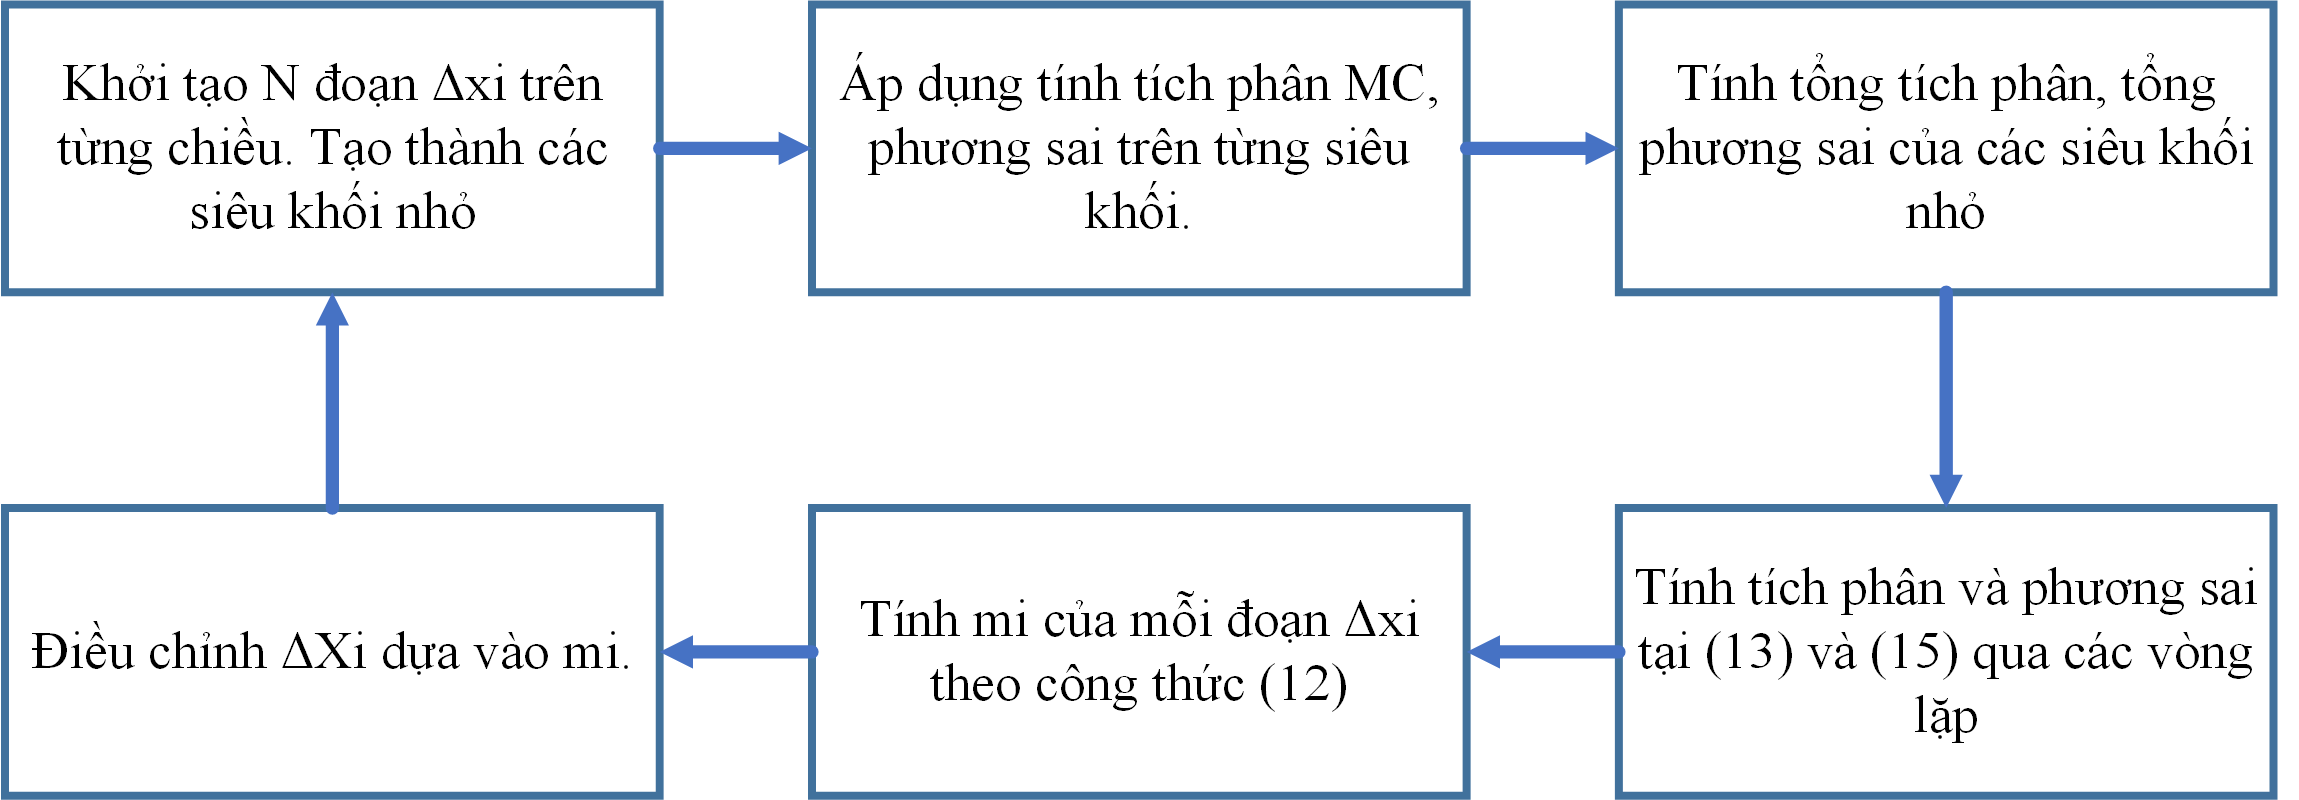
\includegraphics[width=1\textwidth]{flowchar.png}
    \caption{Sơ đồ thuật toán}\label{hinh3.2}
\end{figure}
\end{frame}


\begin{frame}{Kết quả đạt được}\vspace{4pt}
  \textbf{Xét các hàm 1 chiều}\\
  \vspace{0.4em}
\begin{align}
        I=\int_{0}^{1}\frac{dx}{(x-0.25)^2 +10^{-6}}+\frac{dx}{(x-0.5)^2 +10^{-6}}+\frac{dx}{(x-0.75)^2 +10^{-6}}
    \end{align}
    \begin{figure}[H]
        \centering
        \includegraphics[width=0.4\textwidth]{1d_x02505075.png}
        \caption{Dạng đồ thị của f(x)}\label{hinh3.2}
    \end{figure}
\end{frame}

\begin{frame}{Kết quả đạt được}\vspace{4pt}
  \textbf{Xét các hàm 1 chiều}\\
  \vspace{0.4em}
    \begin{table}[H]
        \centering
        \begin{tabular}{ |c|c|c|c|c| }
         \hline
         \multicolumn{1}{|c}{Số mẫu} & \multicolumn{1}{|c|}{Số vòng lặp} & \multicolumn{1}{|c|}{Kết quả I} & \multicolumn{1}{|c|}{Sai số $\sigma$} & \multicolumn{1}{|c|}{Kết quả giải tích số} \\
         \hline
         10000 & 1  & 9370.37 & 29.30 & 9410.11 \\
         \hline
         10000 & 10  & 9410.12 & 0.07 & 9410.11 \\
         \hline
         10000 & 100  & 9410.12 & 0.02 & 9410.11 \\
         \hline
        \end{tabular}
        \caption{Bảng kết quả tích phân 1 chiều}
        \label{1d_x02505075}
       \end{table}

\end{frame}

%%%
\begin{frame}{Kết quả đạt được}\vspace{4pt}
  \textbf{Xét các hàm 1 chiều}\\
  \vspace{0.4em}
  Xét hàm f(x) có đỉnh nhọn cao và hẹp, lấy tích phân trên miền xác định $[10^{-10},2]$
  \begin{align}
      I = \int_{10^{-10}}^{1}\left({\frac{1}{x}+20exp(-10^{-4}(x-1)^2)}\right)dx
  \end{align}
  \begin{figure}[H]
      \centering
      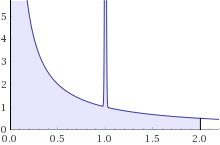
\includegraphics[width=0.4\textwidth]{1d_20.png}
      \caption{Dạng đồ thị của f(x)}\label{hinh3.2}
  \end{figure}
\end{frame}

\begin{frame}{Kết quả đạt được}\vspace{4pt}
  \textbf{Xét các hàm 1 chiều}\\
  \vspace{0.4em}
  \begin{table}[H]
    \centering
    \begin{tabular}{ |c|c|c|c|c| }
     \hline
     \multicolumn{1}{|c}{Số mẫu} & \multicolumn{1}{|c|}{Số vòng lặp} & \multicolumn{1}{|c|}{Kết quả I} & \multicolumn{1}{|c|}{Sai số $\sigma$} & \multicolumn{1}{|c|}{Kết quả giải tích số} \\
     \hline
     10000 & 1  & 11.4698 & 0.6 & $log(2.10^2) + 2.sqrt(\frac{\pi}{10})$ \\
     \hline
     10000 & 10  & 24.0734 & 0.0002 & $log(2.10^2) + 2.sqrt(\frac{\pi}{10})$ \\
     \hline
     10000 & 100  & 24.0734 & 4.039e-05 & $log(2.10^2) + 2.sqrt(\frac{\pi}{10})$ \\
     \hline
    \end{tabular}
    \caption{Bảng kết quả tích phân 1 chiều}
    \label{1d_x02505075}
   \end{table}
\end{frame}

\begin{frame}{Kết quả đạt được}\vspace{4pt}
  \textbf{Xét các hàm hai chiều}\\
  \vspace{0.4em}
  \begin{align}
    I=\int_{-1}^{1}\int_{-1}^{1} {exp(-20(x^2+y^2))}dxdy
\end{align}

\begin{table}[H]
    \centering
    \begin{tabular}{ |c|c|c|c|c| }
     \hline
     \multicolumn{1}{|c}{Số mẫu} & \multicolumn{1}{|c|}{Số vòng lặp} & \multicolumn{1}{|c|}{Kết quả I} & \multicolumn{1}{|c|}{Sai số $\sigma$} & \multicolumn{1}{|c|}{Kết quả giải tích số} \\
     \hline
     10000 & 1  & 0.157403  & 0.0003 & $\approx 0.15708$ \\
     \hline
     10000 & 10  &  0.157029 & 0.0002 & $\approx 0.15708$ \\
     \hline
     10000 & 100  & 0.156698 & 0.0001 & $\approx 0.15708$ \\
     \hline
    \end{tabular}
    \caption{Bảng kết quả tích phân 2 chiều}
    \label{2d_xy}
   \end{table}
\end{frame}


\begin{frame}{Kết quả đạt được}\vspace{4pt}
  \textbf{Xét các hàm ba chiều}\\
  \vspace{0.4em}
  \begin{align}
    I=\int_{0}^{1}\int_{0}^{1} \int_{0}^{1} {\frac{1}{xyz+10^{-6}}}dxdydt
\end{align}
\begin{table}[H]
    \centering
    \begin{tabular}{ |c|c|c|c|c| }
     \hline
     \multicolumn{1}{|c}{Số mẫu} & \multicolumn{1}{|c|}{Số vòng lặp} & \multicolumn{1}{|c|}{Kết quả I} & \multicolumn{1}{|c|}{Sai số $\sigma$} & \multicolumn{1}{|c|}{Kết quả giải tích số} \\
     \hline
     10000 & 1  & 574.415  & 125.527 & 462.216 \\
     \hline
     10000 & 10  & 461.803  & 0.425806 & 462.216 \\
     \hline
     10000 & 100  & 462.31 & 0.0964302 & 462.216 \\
     \hline
    \end{tabular}
    \caption{Bảng kết quả tích phân 3 chiều}
    \label{3d_xyz}
   \end{table}
\end{frame}

\begin{frame}{Kết quả đạt được}\vspace{4pt}
  \textbf{Xét các hàm bốn chiều}\\
  \vspace{0.4em}
  \begin{align}
    I^n=\left(\frac{1}{a{\pi}^{\frac{1}{2}}}\right)^n\int_{0}^{1} 
    {d^nx\exp\left({-\sum_{i=1}^n{\frac{(x_i-0.5)^2}{a^2}}}\right)}
\end{align}
Với $n=4, a=0.1$
\begin{table}[H]
    \centering
    \begin{tabular}{ |c|c|c|c|c| }
     \hline
     \multicolumn{1}{|c}{Số mẫu} & \multicolumn{1}{|c|}{Số vòng lặp} & \multicolumn{1}{|c|}{Kết quả I} & \multicolumn{1}{|c|}{Sai số $\sigma$} & \multicolumn{1}{|c|}{Kết quả giải tích số} \\
     \hline
     10000 & 1  &  1.18126 & 0.1271 & 1 \\
     \hline
     10000 & 10  & 1.00069 & 0.00126 & 1 \\
     \hline
     10000 & 100  & 0.999867 & 0.0004 & 1 \\
     \hline
    \end{tabular}
    \caption{Bảng kết quả tích phân 4 chiều}
    \label{4d_xyzt}
   \end{table}
\end{frame}

%két luân
\begin{frame}{Kết luận và hướng phát triển}\vspace{4pt}
  \textbf{Kết luận}\\
  \vspace{0.4em}
  - Kết quả ước tính tích phân so với kết quả chính xác từ phương pháp giải tích số gần như bằng nhau. \\
  - Xử lý tốt các bài toán có hàm lấy tích phân có hành xử xấu và trong không gian nhiều chiều.\\
\end{frame}
%Hpt
\begin{frame}{Kết luận và hướng phát triển}\vspace{4pt}
  \textbf{Hướng phát triển}\\
  \vspace{0.4em}
  - Tối ưu khả năng tính toán các tích phân lớn hơn 4 chiều.\\
  - Tìm hiểu các thuật toán khác để so sánh kết quả và áp dụng để cải thiện kết quả.\\
\end{frame}

\begin{frame}{}\vspace{4pt}
  \fontsize{16pt}{40pt}
  \textbf{      Cảm ơn quý Thầy Cô và các bạn đã lắng nghe}\\
\end{frame}

\end{document}